\chapter{Lichtablenkung an einem Galaxiencluster\label{chapter:thema}}
\lhead{Lichtablenkung an einem Galaxiencluster}
\begin{refsection}
\chapterauthor{Pascal Stump}

\section{Einleitung}
Der Gravitationslinseneffekt ist ein faszinierender blaber.  Im Bild
\ref{fig:lrg3-757} ist dieser Effekt bei perfekt zu sehen.  Solche
nennt man Einsteinringe.

\begin{figure}
  \centering
  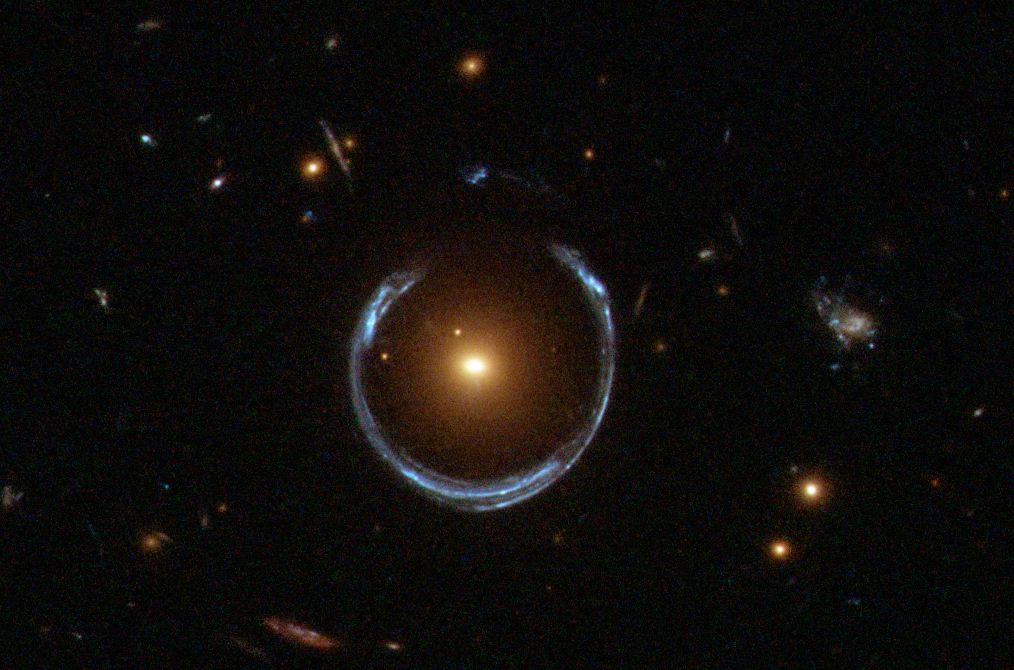
\includegraphics[width=\textwidth]{cluster/images/LRG_3-757}
  \caption{Einsteinring (LRG 3-757; ESA/Hubble \& NASA)}
  \label{fig:lrg3-757}
\end{figure}

\section{``Normale'' Linse}
Bevor Gravitationslinsen behandelt werden, soll hier zuerst einmal ein
Rückblick gegeben werden, wie eine ``normale'' Linse funktioniert.

Eine ``normale'' Linse funktioniert durch Brechung am Übergang
zwischen Umgebung und Linsenmaterial.  Durch die Brechung kommt es zu
einer Winkeländerung.  Welche mit der folgende Formel aus der
geometrischen Optik berechnet werden kann.

\begin{equation}
  \frac{\sin \varepsilon_1}{\sin \varepsilon_2} = \frac{n_2}{n_1}
\end{equation}

Darin kommen die Winkel zur Oberflächennormalen auf der einen Seite
und die beiden Brechungsindizes auf der anderen vor.  Der
Brechungsindex eines Mediums \(n\), ergibt sich aus der
Lichtgeschwindigkeit im Vakuum \(c\) geteilt durch die
Lichtgeschwindigkeit im Medium \(u\).

\begin{equation}
  n = \frac{c}{u}
\end{equation}

Sehr anschaulich wird dies im Prinzip von Hyugens gezeigt.  Nimmt man
eine parallele Wellenfront (siehe Bild \ref{fig:huygens1}) breitet
sich diese in der Zeit \(\Delta t\) immer im gleichen Abstand von
einer Wellenfront zur nächsten aus.  Von jedem Raumpunkt auf einer
``Zeitlinie'' aus, bewegt sich die Lichtwelle eine gewisse Distanz (im
Bild als Halbkreise angedeutet).  Wird nun eine Umhüllende um die
Halbkreise gelegt, erhält man die Position der Lichtwelle zum neuen
Zeitpunkt.

\begin{figure}
  \centering
  %
% Brechung nach dem Prinzip von Huygens


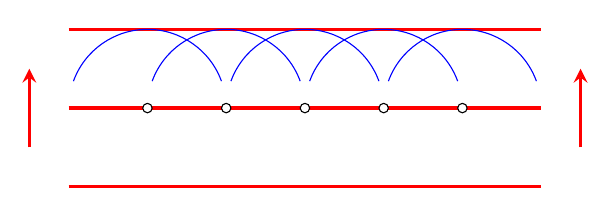
\begin{tikzpicture}

  
  % Delta t
  \foreach \y in {-1,0,1}
    \draw [very thick, color=red] (0,\y) -- (6,\y);

  \foreach \x in {1,2,3,4,5}
    \draw [black, fill=white] (\x,0) circle (.6mm);

  \foreach \x in {1,2,3,4,5}
    \draw [blue] (\x,0) ++ (0,1) arc (90:160:1cm)
                 (\x,0) ++ (0,1) arc (90:20:1cm);

  \draw [very thick, color=red, ->, >=stealth] (-.5,-.5) -- (-.5,0.5);
  \draw [very thick, color=red, ->, >=stealth] (6.5,-.5) -- (6.5,0.5);


\end{tikzpicture}
  \caption{Lichtwellen Ausbreitung nach dem Prinzip von Huygens.}
  \label{fig:huygens1}
\end{figure}

Trifft nun eine solche Wellenfront auf ein Medium mit veränderter
Lichtgeschwindigkeit, so wir die Wellenfront abgelenkt.  Im Bild
\ref{fig:huygens2} ist diese Brechung bei zwei homogenen Medien
aufgezeigt.  Der erste Teil der Wellenfront trifft im Punkt \(A\) auf
den Grenzbereich beider Medien.  Die andere Seite der Wellenfront ist
im Punkt \(B\) und somit noch nicht am Grenzbereich.  Während der
Zeit, die die Wellenfront von \(B\) zum Grenzbereich im Punkt \(D\)
benötigt, legt sie im anderen Medium nur den Weg von \(A\) zu \(C\)
zurück.  Die Wellenfront wurde durch die verringerte
Wellengeschwindigkeit im neuen Medium abgelenkt.

\begin{figure}
  \centering
  %
% Brechung nach dem Prinzip von Huygens


\begin{tikzpicture}
  [every label/.style={color=black}]

  
  % Oberfläche
  \fill [fill=blue!15!white] (0,0) rectangle (6,-2);
  \draw [thick] (0,0) -- (6,0);
  \coordinate[label=below left:$A$] (A) at (3,0);
  \path (A) ++ (2,0) coordinate[label=below right:$D$] (D);

  \draw [very thick, color=red, -<, >=stealth] (A) --++ (150:2.5) node(ray1Start){};
  \path [name path=rayStart] (ray1Start.center) --++ (60:2.5);
  \path [name path=ray2] (A) ++ (2,0) --++ (150:6);
  \draw [very thick, color=red, name intersections={of=rayStart and ray2,
    by=ray2Start}, -<, >=stealth] (A) ++ (2,0) -- (ray2Start);

  \path (ray2Start) ++ (-30:2.5) coordinate[label=above:$B$] (B);
  \draw [color=red] (A) -- (B);


  \draw [thick, color=blue] (A) ++ (.8,0) arc (0:-180:.8cm);
  \draw [thick, color=blue]
    let \p1 = ($(B)-(D)$)
    in (B) ++ (-30:{veclen(\x1,\y1)}) arc (-30:140:{veclen(\x1,\y1)})
       (B) ++ (150:{veclen(\x1,\y1)}) coordinate (Bs)
       (A) ++ (150:{veclen(\x1,\y1)}) coordinate (As);

  \draw [color=red] (As) -- (Bs);

  \node [circle] (circleSmall) at (A) [minimum size=2*.8cm,
    inner sep=0]{};
  \draw [color=red] (D) -- (tangent cs:node=circleSmall, point={(D)},
    solution=2) coordinate[label=below left:$C$] (C);


  \path (C) ++ ($ (C)-(A) $) coordinate (Cs);
  \path (D) ++ ($ (C)-(A) $) coordinate (Ds);
  \draw [very thick, color=red, ->, >=stealth] (A) -- (C) -- ($ (C)!1.4!(Cs) $);
  \draw [very thick, color=red, ->, >=stealth] (D) -- ($ (D)!1.4!(Ds) $);
  \draw [color=red] (Cs) -- (Ds);

  \foreach \point in {A,B,C,D}
    \draw [black, fill=white] (\point) circle (.6mm);


\end{tikzpicture}
  \caption{Brechung nach dem Prinzip von Huygens.}
  \label{fig:huygens2}
\end{figure}

Nun ist es natürlich so, dass es im Weltall keine starr begrenzte
Bereiche gibt, wie in einer gewöhnlichen Linse.  Den Effekt der
Brechung findet jedoch auch in einem inhomogenen Material statt.  Das
Bild \ref{fig:huygens3} soll dies aufzeigen.  Dabei ist die blaue
Fläche die Region mit tieferer Wellengeschwindigkeit.  Dies
veranschaulicht auch, warum sich Lichtstrahlen in Richtung eines
massenhaften Körpers biegen.

\begin{figure}
  \centering
  %
% Brechung nach dem Prinzip von Huygens


\begin{tikzpicture}
  [every label/.style={color=black}]

  
  %

  \shade [inner color=blue!50!white, outer color=white] (-.6,0.55) circle (1.5cm);

  \coordinate (A) at (0,0);
  \coordinate (B) at (3,0);
  \draw [very thick, color=red] (A) -- (B);

  \path (B) ++ (97:1cm) coordinate (Bs);
  \path (Bs) ++ ($ (A)!1!187:(B) $) coordinate (As);
  \draw [very thick, color=red] (As) -- (Bs);

  \path (Bs) ++ (104:1cm) coordinate (Bss);
  \path (Bss) ++ ($ (A)!1!194:(B) $) coordinate (Ass);
  \draw [very thick, color=red] (Ass) -- (Bss);

  \draw [very thick, color=red] (A) ++ (0,-1) --++ ($ (B)-(A) $);
  \draw [very thick, color=red] (Bss) ++ (104:1cm) --++ ($ (A)!1!194:(B) $);

  
  % \fill [fill=blue!15!white] (0,0) rectangle (6,-2);
  % \draw [thick] (0,0) -- (6,0);
  % \coordinate[label=below left:$A$] (A) at (3,0);
  % \path (A) ++ (2,0) coordinate[label=below right:$D$] (D);

  % \draw [very thick, color=red, -<, >=stealth] (A) --++ (150:2.5) node(ray1Start){};
  % \path [name path=rayStart] (ray1Start.center) --++ (60:2.5);
  % \path [name path=ray2] (A) ++ (2,0) --++ (150:6);
  % \draw [very thick, color=red, name intersections={of=rayStart and ray2,
  %   by=ray2Start}, -<, >=stealth] (A) ++ (2,0) -- (ray2Start);

  % \path (ray2Start) ++ (-30:2.5) coordinate[label=above:$B$] (B);
  % \draw [color=red] (A) -- (B);


  % \draw [thick, color=blue] (A) ++ (.8,0) arc (0:-180:.8cm);
  % \draw [thick, color=blue]
  %   let \p1 = ($(B)-(D)$)
  %   in (B) ++ (-30:{veclen(\x1,\y1)}) arc (-30:140:{veclen(\x1,\y1)})
  %      (B) ++ (150:{veclen(\x1,\y1)}) coordinate (Bs)
  %      (A) ++ (150:{veclen(\x1,\y1)}) coordinate (As);

  % \draw [color=red] (As) -- (Bs);

  % \node [circle] (circleSmall) at (A) [minimum size=2*.8cm,
  %   inner sep=0]{};
  % \draw [color=red] (D) -- (tangent cs:node=circleSmall, point={(D)},
  %   solution=2) coordinate[label=below left:$C$] (C);


  % \path (C) ++ ($ (C)-(A) $) coordinate (Cs);
  % \path (D) ++ ($ (C)-(A) $) coordinate (Ds);
  % \draw [very thick, color=red, ->, >=stealth] (A) -- (C) -- ($ (C)!1.4!(Cs) $);
  % \draw [very thick, color=red, ->, >=stealth] (D) -- ($ (D)!1.4!(Ds) $);
  % \draw [color=red] (Cs) -- (Ds);

  % \foreach \point in {A,B,C,D}
  %   \draw [black, fill=white] (\point) circle (.6mm);


\end{tikzpicture}
  \caption{Brechung nach dem Prinzip von Huygens in einem inhomogen
    Material.}
  \label{fig:huygens3}
\end{figure}



\begin{figure}
  \centering
  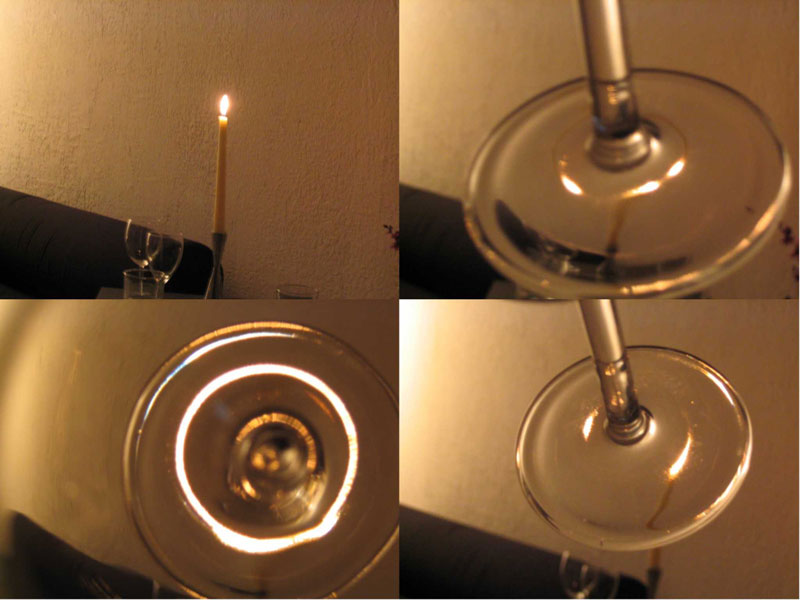
\includegraphics[width=\textwidth]{cluster/images/model_grav_lens}
  \caption{Model einer Gravitationslinse (Boden eines Weinglases)
    \cite{standford:ModelGravLens}}
  \label{fig:ModelGravLinse}
\end{figure}

\printbibliography[heading=subbibliography]
\end{refsection}

